\documentclass[twocolumn]{article}

\usepackage{array}
\usepackage[autocite=superscript]{biblatex}
\usepackage{booktabs}
%\usepackage[margin=0.75in]{geometry}
\usepackage{graphicx}
\usepackage{multicol}
\usepackage{multirow}
\usepackage{nopageno}
\usepackage{tabularx}
\usepackage{units}

\addbibresource{curated_refs.bib}

\usepackage{fontspec}
\setmainfont{Liberation Sans}

\graphicspath{
 {figure_1/}
 {figure_2/}
 {figure_3/}
 {figure_4/}
}

\setcounter{secnumdepth}{0}

\newcommand\captitle{\textit}
\newcommand\reffig[1]{Figure \ref{#1}}
\newcommand\reftab[1]{Table \ref{#1}}
\newcommand\seq[1]{\texttt{#1}}

\newcommand\latin[1]{\emph{#1}}
\newcommand\apo{\latin{apo}}
\newcommand\holo{\latin{holo}}
\newcommand\invitro{\latin{in vitro}}
\newcommand\invivo{\latin{in vivo}}

\newcommand\hr[1]{\unit[#1]{h}}
\newcommand\mgml[1]{\unit[#1]{mg/mL}}
\newcommand\minx[1]{\unit[#1]{min}}
\newcommand\mm[1]{\unit[#1]{mM}}
\newcommand\ngx[1]{\unit[#1]{ng}}
\newcommand\ngul[1]{\unit[#1]{ng/μL}}
\newcommand\nm[1]{\unit[#1]{nM}}
\newcommand\px[1]{\unit[#1]{px}}
\newcommand\ul[1]{\unit[#1]{μL}}
\newcommand\um[1]{\unit[#1]{μM}}
\newcommand\uul[1]{\unit[#1]{U/μL}}
\newcommand\vcm[1]{\unit[#1]{V/cm}}

\newcommand\beginsupplement{%
   \setcounter{table}{0}
   \renewcommand{\thetable}{S\arabic{table}}%
   \setcounter{figure}{0}
   \renewcommand{\thefigure}{S\arabic{figure}}%
}

\begin{document}

\begin{figure}
 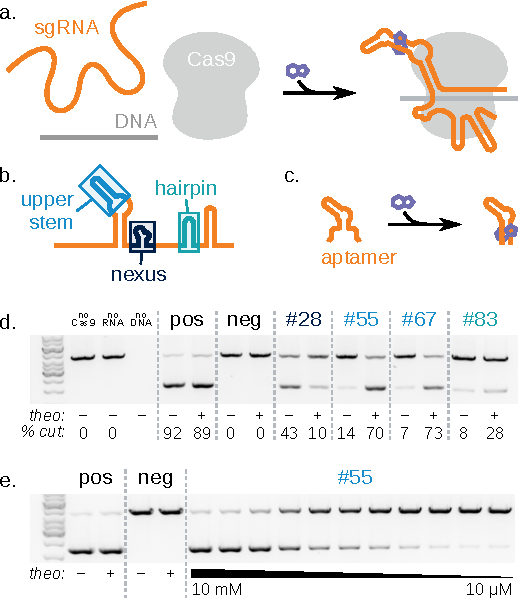
\includegraphics[width=\columnwidth]{figure_1}
 \caption{
  \captitle{Rational design of ligand-sensitive sgRNAs}
  (a) A schematic illustrating that our ligand-activated designs are meant to 
  adopt the native sgRNA fold upon the addition of ligand, which then allows 
  for the assembly of a functional Cas9 complex.
  (b) A map of the sgRNA domains most relevant to this paper 
  \autocite{briner2014}.
  (c) The mechanism by which the theophylline aptamer can affect conformational 
  change in an RNA device.  In the absence of ligand, the ends of the aptamer 
  are unstructured.  In the presence of ligand, the ends come together to form 
  a rigid stem-like structure \autocite{zimmerman1997}.
  (d) \emph{In vitro} cleavage with and without theophylline for some of our 
  strongest rational designs.  From left to right: Leaving Cas9 or sgRNA out of 
  the reaction leads to no cleavage, and leaving DNA out of the reaction leads 
  to no signal.  The positive and negative controls are unaffected by 
  theophylline.  Design numbers refer to Table S1 and are color-coded by the 
  domain in which the aptamer was inserted.  The percent cleavage values are 
  the average of at least two experiments.  All data in the image is from a 
  single gel, but several weaker designs were cropped.
  (e) Theophylline titration for design \#55.  The theophylline concentration 
  decreases by 2x in each step of the titration.
 }
 \label{fig1}
\end{figure}

\begin{table}
 \centering
 \resizebox{\columnwidth}{!}{\begin{tabular}{llrrr}
\toprule
\bfseries Strategy &
\bfseries Domain &
\begin{tabular}{@{}r@{}}\bfseries \# Tested \\ \bfseries Designs\end{tabular} &
\begin{tabular}{@{}r@{}}\bfseries \# Active \\ \bfseries Designs\end{tabular} &
\begin{tabular}{@{}r@{}}\bfseries Best      \\ \bfseries Activity\end{tabular} \\
\midrule
    Stem Replacement
        & Upper Stem & 20 & 2 & 18\% \\
        & Lower Stem & 5 & 0 &  \\
        & Nexus & 14 & 1 & -32\% \\
        & Hairpin & 5 & 0 &  \\
    \midrule
    Induced Dimerization
        & Upper Stem & 5 & 0 &  \\
    \midrule
    Strand displacement
        & Upper Stem & 20 & 4 & 67\% \\
        & Lower Stem & 10 & 0 &  \\
        & Hairpin & 16 & 3 & 20\% \\
\bottomrule
\end{tabular}}
 \caption{
  \captitle{Summary of rational design results.}  The results are organized by 
  the design strategy we employed and the domain the sgrNA was inserted into.  
  We tested 97 designs and found 10 that were active, including at least one 
  active design for each domain.  We considered a design active if it exhibited 
  a >15% change in cleavage in response to theophylline; 15% is about the point 
  at which the difference is clearly visible on a gel.
 }
 \label{tab1}
\end{table}

\section{Methods}

\subsection{\latin{In vitro} Cas9 cleavage assay}

\latin{In vitro} transcription: Linear, double-stranded template DNA was 
acquired either by ordering gBlocks® Gene Fragments from IDT (\reffig{fig1}) or 
by digesting plasmid DNA with EcoRI and HindIII (\reffig{fig2}).  Each 
construct had the following T7 promoter --- \seq{TATAGTAATAATACGACTCACTATAG} 
--- and a spacer sequence that began with at least 3 G's.  The HiScribe™ T7 
High Yield RNA Synthesis Kit from NEB (E2040S) was used to transcribe 
\ngx{10-50} of DNA template, and the RNA Clean \& Concentrator™-25 spin columns 
from Zymo (R1018) were used to remove unincorporated nucleotides.  The RNA was 
diluted to \nm{1500} (as measured by NanoDrop) in nuclease-free water from 
Ambion (9983), aliquoted, and stored at -80°C.  

Target DNA: Target DNA was prepared by using inverse PCR to clone the 
appropriate target sequence into the pCR2.1 vector roughly across from the XmnI 
site (i.e. in the MCS).  The vector was then digested with XmnI from NEB 
(R0194S): mix \ul{43.5} \ngul{≈500} miniprepped pCR2.1 DNA, \ul{5.0} 10x 
CutSmart buffer, and \ul{1.5} \uul{20} XmnI; incubate at 37°C until no 
uncleaved plasmid is detectable on a gel (usually \hr{1-2}); dilute to \nm{30}; 
store at -20°C.  

Cas9 reaction: Mix \ul{5.0} water or \mm{30} theophylline and \ul{1.5} \um{1.5}
sgRNA; incubate at 95°C for \minx{3}, then at 4°C for \minx{1}; add \ul{5.48} 
water, \ul{1.5} 10x Cas9 buffer, and \ul{0.02} \um{20} Cas9 (NEB, M0386T) via 
master mix; incubate at room temperature for \minx{10}; add \ul{1.5} \nm{30} 
target DNA; pipet to mix; incubate at 37°C for \hr{1}; add \ul{0.09} \mgml{20} 
RNase~A (Sigma, R6148), \ul{0.09} \mgml{20} Proteinase~K (Denville, CB3210-5), 
and \ul{2.82} 6x loading dye via master mix; incubate at 37°C for \minx{20}, 
then at 55°C for \minx{20}; run the entire reaction (\ul{18}) on a 1\% 
agarose/TAE/GelRed gel at \vcm{4.5} for \minx{70}.  The exposure time was 
manually adjusted to be as long as possible without saturating any pixels.

Gel quantification: Open gel in ImageJ (1.51r); subtract the background with a 
rolling ball radius of \px{50}; then analyze the gel bands as usual.  The 
percent cleavage for each lane was calculated:

\begin{displaymath}
 \mathrm{f} = \frac{\mathrm{pixels}_\mathrm{2kb}}{\mathrm{pixels}_\mathrm{4kb} 
 + \mathrm{pixels}_\mathrm{2kb}}
\end{displaymath}

The response to ligand was calculated: 

\begin{displaymath}
 \mathrm{Δf} = \mathrm{f}_\mathrm{theo} - \mathrm{f}_\mathrm{apo}
\end{displaymath}

\subsection{\emph{In vivo} CRISPRi assay}

Dolor sit amet.

\printbibliography[title=References]

\beginsupplement

\

\end{document}
